\chapter{Artificial Neural Networks}



Artificial neural network models of all kinds are the backbone of deep learning mechanics.  A common elementary application is to utilize a network to recognize and classify image date based on the pixel values, as is shown in Figure \ref{minecraft}.  


\begin{figure}[H]
    \centering
    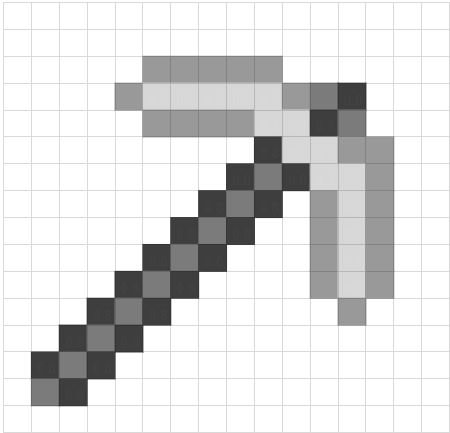
\includegraphics[width=.35\textwidth]{Figures/pickaxe_1.png}
    \hspace{30pt}
    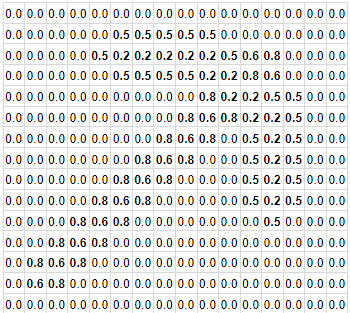
\includegraphics[width=.35\textwidth]{Figures/pickaxe_2.png}
    \caption{\footnotesize{A two-layer neural network}}
    \label{minecraft}
\end{figure}





\section{The Architecture of Neural Networks} %-------------SECTION

Hint toward issues like overfitting, but elaborate more in section 2.3.

- Also, first mention \textbf{Optimization} here

\subfile{Architecture}  % Pathway to Architecture file

%\subsection{Gradient Descent}

%\subsubsection{Simulation in R}

%\subsection{Backpropagation}

%\subsubsection{Simulation in R}

\subsection{More Optimization Algorithms and Activation Functions}

\section{Types of Neural Networks} %-------------SECTION

Write this up in R following along the code from \textbf{RAI}, with supplementary information from other sources as well.  

Obviously not all types will be covered, but here are a few.  

Include \textbf{mathematical notation} for each network mentioned.

\subsection{Multi-Layer Perceptron}
Keras Model: "sequential"

\subsection{Convolutional Neural Networks}
Unstructured image data

\subsection{Generative Adversarial Networks}
Unstructured image data

\subsection{Recurrent Neural Networks}
Unstructured text data

\subsection{Long Short-Term Memory Network}
Unstructured text data

\subsection{Convolutional Recurrent Networks}
Unstructured text data

\section{Techniques to Improve Model Performance} %-------------SECTION

The primary objective in machine learning (and therefore deep learning) is to perform well on new, unseen data. 

- \textbf{Overfitting} and \textbf{underfitting}

\subsection{Rating Model Performance}
- \textbf{Generalization}
- \textbf{Training error}  
- \textbf{Generalization error} (test error)

\subsection{Addressing Model Performance}
- \textbf{Capacity}
- \textbf{Regularization}

\subsection{Common Problems and Relevant Techniques}

Earthquake example